%-------------------------------------------%
%-------------------------------------------%
\section{Poles and Stability}
%-------------------------------------------%
Poles are the solutions of the characteristic equation(the denominator of a transfer function) which defines the stability of the system.\\\\
The impulse response have different look when their poles have different locations in the s-domain.
\begin{itemize}
    \item \textbf{Poles at:} $s = \sigma \pm \mathbf{j}\omega$
    
    \item \textbf{Impulse response:}
    \[ g(t) = Ae^{(\sigma \pm \mathbf{j}\omega)t} = Ae^{\sigma t}(\cos(\omega t)\pm\mathbf{j}\sin(\omega t))\]
    \ where $\omega$ is the frequency of the oscillation.
\end{itemize}

\begin{figure}[H] 
    \centering
    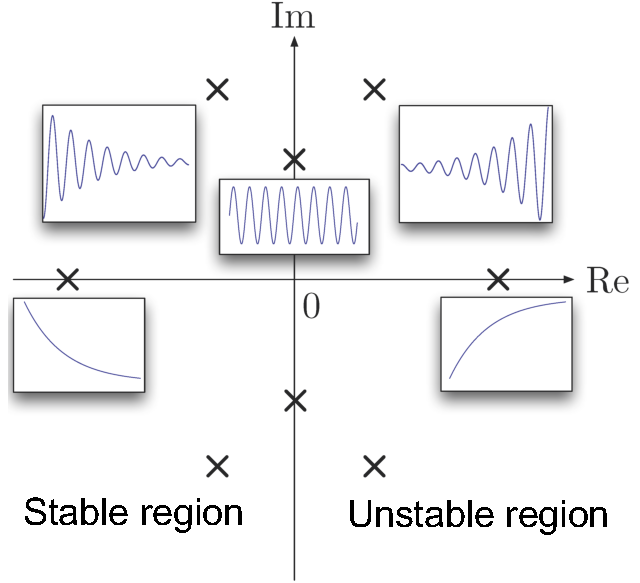
\includegraphics[width=.45\textwidth]{images/pole_location.pdf}
    \caption{Pole location}
\end{figure}

Stability is evaluated by the signs of the real parts of the poles:
\begin{itemize}
    \item \textbf{Asymptotic stability}: when $\Re\{p_{i}\} < 0 $ for all poles $p_{i}$: (\textsc{Fig. 3} - stable region)
        \begin{itemize}
            \item The output decays within an exponential envelope approaching asymptotically 0. 
        \end{itemize}
        
    \item \textbf{Instability} when at least one pole is $\Re\{p_{i}\} >0$: (\textsc{Fig. 3} - unstable region)
        \begin{itemize}
            \item The output grows without bound. 
        \end{itemize}
        
    \item \textbf{Marginal stability} when $\Re\{p_{i}\} =0$ for some poles and $\Re\{p_{i}\} <0$ for all other poles: (\textsc{Fig. 3} - middle)
        \begin{itemize}
            \item The output never decays or grows in amplitude, and shows sustained oscillations. 
        \end{itemize}
\end{itemize}
%-------------------------------------------%
%-------------------------------------------%
\subsection{Finding Stability}
%-------------------------------------------%
We have 2 methods to find the stability of the system:
\begin{enumerate}
    \item \textbf{Solving the characteristic equation} to find poles. The signs of the real part of the poles indicates the stability of the system.
    \item \textbf{Routh stability criterion}. This is particularly useful if the characteristic equation is of high order and tedious to solve.
\end{enumerate}
%*******************************************%

%-------------------------------------------%
\subsubsection{Routh Stability Criterion}
%-------------------------------------------%
Routh Table can determine the number of poles with positive real parts.
\begin{itemize}
\item We only care about the denominator of the transfer function. 
\item Key concept: \textbf{The number of change of sign in the 1st column  = number of poles with positive real parts.}
\end{itemize}
\ \\
\underline{\textbf{To create a Routh Table:}}
\begin{itemize}
\item Given the transfer function:
    \[G(s) = \frac{N(s)}{D(s)}\]
    and 
    \[D(s) = a_{n}s^{n}+a_{n-1}s^{n-1}+\ldots+a_{1}s+a_{0}\]
    
    \item Fill in the corresponding values to the Routh Table:
        \begin{table}[H]
            \centering 
            \begin{tabular}{c|c|c|c}
                 $s^{n}$ & $a^{n}$ & $a^{n-2}$ & $a^{n-4}$\\ \hline
                 $s^{n-1}$ & $a^{n-1}$ & $a^{n-3}$ & $a^{n-5}$\\ \hline \hline
                 $s^{n-2}$ & $b^{(n-2)}_{1}$ & $b^{(n-2)}_{2}$ & $b^{(n-2)}_{3}$ \\ \hline 
                 $s^{n-3}$ & $b^{(n-3)}_{1}$ & $b^{(n-3)}_{2}$ & $b^{(n-3)}_{3}$\\ \hline
                 $\vdots$&$\vdots$&$\vdots$&\\ \hline
                 $s^{2}$ & $b^{(2)}_{1}$ & $b^{(2)}_{2}$ & 0 \\ \hline
                 $s^{1}$ & $b^{(1)}_{1}$ & 0 & \\ \hline
                 $s^{0}$ & $b^{(0)}_{1}$ & &\\ \hline
            \end{tabular}
         \end{table}
         
         \begin{minipage}{.4\textwidth}
         where 
         \[b_{i}^{(k)} = \frac{b_{1}^{(k+1)}\times b_{i+1}^{(k+2)} - b_{1}^{(k+2)}\times b_{i+1}^{(k+1)}}{b_{1}^{(k+1)}}\]
         \end{minipage}\hfill
        \begin{minipage}{.6\textwidth}
            \begin{figure}[H] 
                \centering
                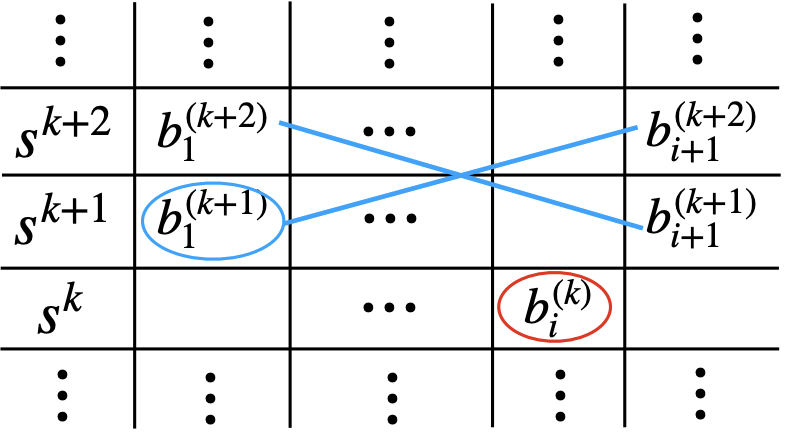
\includegraphics[width=.7\textwidth]{images/routh.png}
            \end{figure}
        \end{minipage}
        
    \item The system is asymptotically stable \textit{if and only if}
        \begin{itemize}
            \item $a_{i}>0 ,\ \forall i$ (for all $i$ values)
            \item \textbf{no change of sign} in the 1st column of the Routh Table.
        \end{itemize}
\end{itemize}
%---------------EXAMPLE---------------%
\begin{ex}{}
Given the transfer function $\displaystyle G(s) = \frac{2s+1}{s^{2}+5s+6}$, evaluate the stability of the system.\\
\begin{minipage}{0.3\textwidth}
     \begin{table}[H]
        \begin{tabular}{c|c|c}
            $s^{2}$&1&6\\ \hline
            $s^{1}$&5&0\\ \hline \hline 
            $s^{0}$&$\frac{6\times 5 -1\times 0}{5}=6$&\\ 
        \end{tabular}
     \end{table}
\end{minipage} \hfill
\begin{minipage}{0.7\textwidth}
 No change of sign in the 1st column since $1\to 5\to 6$. \\ Therefore, it has 0 unstable poles.
 \end{minipage} \ \\ \\
\textit{Note: for the cells with no value from the characteristic function, but this cell is involved in calculation, fill in 0 instead.}
\end{ex}
%----------------EXAMPLE END----------------%
%---------------EXAMPLE START---------------%
\begin{ex}{}
Given the transfer function $\displaystyle G(s) = \frac{2s+1}{s^{3}+s^{2}+3s+10}$, evaluate the poles.\\\\
\begin{minipage}{0.5\textwidth}
    \begin{table}[H]
        \begin{tabular}{c|c|c|c}
            $s^{3}$&1&3&0\\ \hline
            $s^{2}$&1&10&0\\ \hline \hline
            $s^{1}$&$\frac{3\times -1\times 10}{1}=-7$&(\textit{assume}) $x$(=0)& \\ \hline 
            $s^{0}$&$\frac{-7\times 10 -1\times x}{-7}=10$&&\\ 
        \end{tabular}
    \end{table}
 \end{minipage} \hfill
 \begin{minipage}{0.4\textwidth}
    To find the value of $x$:
    \[x = \frac{10\times0-3\times0}{1}=0\]
 \end{minipage}\\\\\\
  It has 2 unstable poles since the sign has changed twice($1\to 1\to -7 \to 10$) in the first column.
  \ \\ \\
 \textit{Note: add a column to the right when necessary.}
\end{ex}
%----------------EXAMPLE END----------------%


%-------------------------------------------%
\subsection{Final Value Theorem}
%-------------------------------------------%
Final value theorem:
\[\lim_{t\to \infty}y(t) = \lim_{s\to 0}sY(s)\]
\ \ where 
\[y(t) = C_{1}e^{p_{1}t} +  C_{2}e^{p_{2}t}+ \ldots +  C_{n}e^{p_{n}t}\]
\ \ and 
\[Y(s) = \frac{C_{1}}{s-p_{1}}+\frac{C_{2}}{s-p_{2}}+\ldots+\frac{C_{n}}{s-p_{n}}\]

\begin{itemize}
    \item \textbf{Constant} when $p_{1}=0$ and all other $p_{i}$ have $\Re (p_{i})<0$. Then the final value is $C_{1}$.
    
    \item \textbf{Undefined} when there are $p_{i}$ on the imaginary axis. Then $y(t)$ oscillates and does not converge.
    
    \item \textbf{Unbounded} when there are any $p_{i}$ with $\Re (p_{i})>0$.
\end{itemize}

%---------------EXAMPLE START---------------%
\begin{ex}{}
    Find the steady state of the \underline{step response} for the system $\displaystyle G(s)=\frac{3}{s-2}$.
    \vspace{.3cm} \hrule \vspace{.3cm}
    If we apply the final value theorem \textit{blindly}:
    \[\lim_{t\to \infty}y(t) = \lim_{s\to 0}sY(s)=\lim_{s\to 0}G(s)=-\frac{3}{2}\]
    \underline{\textbf{This is a wrong answer!!}}
    \\\\
    However, we know that the step response is
    \[Y(s) =U(s)G(s)= \frac{3}{s-2}\frac{1}{s}=\frac{-1.5}{s}+\frac{1.5}{s-2}\]
    Take the inverse Laplace's transform:
    \[y(t) = -\frac{3}{2}+\frac{3}{2}e^{2t}\]
    Therefore
    \[\lim_{t\to \infty}y(t) = \infty\]
    Unbounded, since $\Re (p_{i})>0$ holds for any $p_{i}$.
    \underline{\textbf{This is the correct answer!!}}
\end{ex}
%----------------EXAMPLE END----------------%